\PassOptionsToPackage{unicode=true}{hyperref} % options for packages loaded elsewhere
\PassOptionsToPackage{hyphens}{url}
%
\documentclass[]{article}
\usepackage{lmodern}
\usepackage{amssymb,amsmath}
\usepackage{ifxetex,ifluatex}
\usepackage{fixltx2e} % provides \textsubscript
\ifnum 0\ifxetex 1\fi\ifluatex 1\fi=0 % if pdftex
  \usepackage[T1]{fontenc}
  \usepackage[utf8]{inputenc}
  \usepackage{textcomp} % provides euro and other symbols
\else % if luatex or xelatex
  \usepackage{unicode-math}
  \defaultfontfeatures{Ligatures=TeX,Scale=MatchLowercase}
\fi
% use upquote if available, for straight quotes in verbatim environments
\IfFileExists{upquote.sty}{\usepackage{upquote}}{}
% use microtype if available
\IfFileExists{microtype.sty}{%
\usepackage[]{microtype}
\UseMicrotypeSet[protrusion]{basicmath} % disable protrusion for tt fonts
}{}
\IfFileExists{parskip.sty}{%
\usepackage{parskip}
}{% else
\setlength{\parindent}{0pt}
\setlength{\parskip}{6pt plus 2pt minus 1pt}
}
\usepackage{hyperref}
\hypersetup{
            pdftitle={Time Value of Money},
            pdfauthor={Colin James},
            pdfborder={0 0 0},
            breaklinks=true}
\urlstyle{same}  % don't use monospace font for urls
\usepackage[margin=1in]{geometry}
\usepackage{color}
\usepackage{fancyvrb}
\newcommand{\VerbBar}{|}
\newcommand{\VERB}{\Verb[commandchars=\\\{\}]}
\DefineVerbatimEnvironment{Highlighting}{Verbatim}{commandchars=\\\{\}}
% Add ',fontsize=\small' for more characters per line
\usepackage{framed}
\definecolor{shadecolor}{RGB}{248,248,248}
\newenvironment{Shaded}{\begin{snugshade}}{\end{snugshade}}
\newcommand{\AlertTok}[1]{\textcolor[rgb]{0.94,0.16,0.16}{#1}}
\newcommand{\AnnotationTok}[1]{\textcolor[rgb]{0.56,0.35,0.01}{\textbf{\textit{#1}}}}
\newcommand{\AttributeTok}[1]{\textcolor[rgb]{0.77,0.63,0.00}{#1}}
\newcommand{\BaseNTok}[1]{\textcolor[rgb]{0.00,0.00,0.81}{#1}}
\newcommand{\BuiltInTok}[1]{#1}
\newcommand{\CharTok}[1]{\textcolor[rgb]{0.31,0.60,0.02}{#1}}
\newcommand{\CommentTok}[1]{\textcolor[rgb]{0.56,0.35,0.01}{\textit{#1}}}
\newcommand{\CommentVarTok}[1]{\textcolor[rgb]{0.56,0.35,0.01}{\textbf{\textit{#1}}}}
\newcommand{\ConstantTok}[1]{\textcolor[rgb]{0.00,0.00,0.00}{#1}}
\newcommand{\ControlFlowTok}[1]{\textcolor[rgb]{0.13,0.29,0.53}{\textbf{#1}}}
\newcommand{\DataTypeTok}[1]{\textcolor[rgb]{0.13,0.29,0.53}{#1}}
\newcommand{\DecValTok}[1]{\textcolor[rgb]{0.00,0.00,0.81}{#1}}
\newcommand{\DocumentationTok}[1]{\textcolor[rgb]{0.56,0.35,0.01}{\textbf{\textit{#1}}}}
\newcommand{\ErrorTok}[1]{\textcolor[rgb]{0.64,0.00,0.00}{\textbf{#1}}}
\newcommand{\ExtensionTok}[1]{#1}
\newcommand{\FloatTok}[1]{\textcolor[rgb]{0.00,0.00,0.81}{#1}}
\newcommand{\FunctionTok}[1]{\textcolor[rgb]{0.00,0.00,0.00}{#1}}
\newcommand{\ImportTok}[1]{#1}
\newcommand{\InformationTok}[1]{\textcolor[rgb]{0.56,0.35,0.01}{\textbf{\textit{#1}}}}
\newcommand{\KeywordTok}[1]{\textcolor[rgb]{0.13,0.29,0.53}{\textbf{#1}}}
\newcommand{\NormalTok}[1]{#1}
\newcommand{\OperatorTok}[1]{\textcolor[rgb]{0.81,0.36,0.00}{\textbf{#1}}}
\newcommand{\OtherTok}[1]{\textcolor[rgb]{0.56,0.35,0.01}{#1}}
\newcommand{\PreprocessorTok}[1]{\textcolor[rgb]{0.56,0.35,0.01}{\textit{#1}}}
\newcommand{\RegionMarkerTok}[1]{#1}
\newcommand{\SpecialCharTok}[1]{\textcolor[rgb]{0.00,0.00,0.00}{#1}}
\newcommand{\SpecialStringTok}[1]{\textcolor[rgb]{0.31,0.60,0.02}{#1}}
\newcommand{\StringTok}[1]{\textcolor[rgb]{0.31,0.60,0.02}{#1}}
\newcommand{\VariableTok}[1]{\textcolor[rgb]{0.00,0.00,0.00}{#1}}
\newcommand{\VerbatimStringTok}[1]{\textcolor[rgb]{0.31,0.60,0.02}{#1}}
\newcommand{\WarningTok}[1]{\textcolor[rgb]{0.56,0.35,0.01}{\textbf{\textit{#1}}}}
\usepackage{graphicx,grffile}
\makeatletter
\def\maxwidth{\ifdim\Gin@nat@width>\linewidth\linewidth\else\Gin@nat@width\fi}
\def\maxheight{\ifdim\Gin@nat@height>\textheight\textheight\else\Gin@nat@height\fi}
\makeatother
% Scale images if necessary, so that they will not overflow the page
% margins by default, and it is still possible to overwrite the defaults
% using explicit options in \includegraphics[width, height, ...]{}
\setkeys{Gin}{width=\maxwidth,height=\maxheight,keepaspectratio}
\setlength{\emergencystretch}{3em}  % prevent overfull lines
\providecommand{\tightlist}{%
  \setlength{\itemsep}{0pt}\setlength{\parskip}{0pt}}
\setcounter{secnumdepth}{0}
% Redefines (sub)paragraphs to behave more like sections
\ifx\paragraph\undefined\else
\let\oldparagraph\paragraph
\renewcommand{\paragraph}[1]{\oldparagraph{#1}\mbox{}}
\fi
\ifx\subparagraph\undefined\else
\let\oldsubparagraph\subparagraph
\renewcommand{\subparagraph}[1]{\oldsubparagraph{#1}\mbox{}}
\fi

% set default figure placement to htbp
\makeatletter
\def\fps@figure{htbp}
\makeatother

\usepackage{etoolbox}
\makeatletter
\providecommand{\subtitle}[1]{% add subtitle to \maketitle
  \apptocmd{\@title}{\par {\large #1 \par}}{}{}
}
\makeatother

\title{Time Value of Money}
\author{Colin James}
\date{2020-07-26}

\begin{document}
\maketitle

\hypertarget{time-value-of-money}{%
\subsubsection{Time Value of Money}\label{time-value-of-money}}

Understanding the time value of money is essential to finance. The value
of something is not a static but dynamic thing. Dating back as far as
5000 BC, this concept is the foundation of modern day finance
(\url{https://www.encyclopedia.com/finance/encyclopedias-almanacs-transcripts-and-maps/time-value-money}).
Thankfully R makes calculations for TVM easy and efficient. TVM
calculations are broken down into 4 topicsL Future Value, Present Value,
Rates of Return and Amortization.

\begin{Shaded}
\begin{Highlighting}[]
\CommentTok{#install.packages("modelr")}
\CommentTok{#install.packages("FinCal")}
\CommentTok{#install.packages("dplyr")}
\CommentTok{#install.packages("FinancialMath")}

\KeywordTok{library}\NormalTok{(}\StringTok{"modelr"}\NormalTok{)}
\KeywordTok{library}\NormalTok{(}\StringTok{"FinCal"}\NormalTok{)}
\KeywordTok{library}\NormalTok{(}\StringTok{"dplyr"}\NormalTok{)}
\end{Highlighting}
\end{Shaded}

\begin{verbatim}
## 
## Attaching package: 'dplyr'
\end{verbatim}

\begin{verbatim}
## The following objects are masked from 'package:stats':
## 
##     filter, lag
\end{verbatim}

\begin{verbatim}
## The following objects are masked from 'package:base':
## 
##     intersect, setdiff, setequal, union
\end{verbatim}

\begin{Shaded}
\begin{Highlighting}[]
\KeywordTok{library}\NormalTok{(}\StringTok{"FinancialMath"}\NormalTok{)}
\KeywordTok{library}\NormalTok{(}\StringTok{"ggplot2"}\NormalTok{)}
\end{Highlighting}
\end{Shaded}

\hypertarget{future-value-and-present-value}{%
\subsection{Future Value and Present
Value}\label{future-value-and-present-value}}

\begin{Shaded}
\begin{Highlighting}[]
\CommentTok{#Below is random cash flow data I have added for these exercises.  We are going to assume our invesment period is 8 years, interest is 10%, and this is an ordinary annunity}
\NormalTok{cash_flow <-}\StringTok{ }\KeywordTok{c}\NormalTok{(}\OperatorTok{-}\DecValTok{10023}\NormalTok{,}\OperatorTok{-}\DecValTok{84949}\NormalTok{,}\OperatorTok{-}\DecValTok{84940}\NormalTok{,}\OperatorTok{-}\DecValTok{83838}\NormalTok{,}\OperatorTok{-}\DecValTok{93838}\NormalTok{,}\OperatorTok{-}\DecValTok{73839}\NormalTok{,}\OperatorTok{-}\DecValTok{83383}\NormalTok{,}\OperatorTok{-}\DecValTok{102939}\NormalTok{)}

\NormalTok{i =}\StringTok{ }\FloatTok{1.10}
\CommentTok{#Manual calculation of FV}
\NormalTok{(cash_flow[}\DecValTok{1}\NormalTok{] }\OperatorTok{*}\StringTok{ }\NormalTok{i }\OperatorTok{^}\StringTok{ }\DecValTok{7}\NormalTok{) }\OperatorTok{+}\StringTok{ }\NormalTok{(cash_flow[}\DecValTok{2}\NormalTok{] }\OperatorTok{*}\StringTok{ }\NormalTok{i }\OperatorTok{^}\StringTok{ }\DecValTok{6}\NormalTok{)  }\OperatorTok{+}\StringTok{  }\NormalTok{(cash_flow[}\DecValTok{3}\NormalTok{] }\OperatorTok{*}\StringTok{ }\NormalTok{i }\OperatorTok{^}\StringTok{ }\DecValTok{5}\NormalTok{) }\OperatorTok{+}\StringTok{ }\NormalTok{(cash_flow[}\DecValTok{4}\NormalTok{] }\OperatorTok{*}\StringTok{ }\NormalTok{i }\OperatorTok{^}\StringTok{ }\DecValTok{4}\NormalTok{) }\OperatorTok{+}\StringTok{ }\NormalTok{(cash_flow[}\DecValTok{5}\NormalTok{] }\OperatorTok{*}\StringTok{ }\NormalTok{i }\OperatorTok{^}\StringTok{ }\DecValTok{3}\NormalTok{) }\OperatorTok{+}\StringTok{ }\NormalTok{(cash_flow[}\DecValTok{6}\NormalTok{] }\OperatorTok{*}\StringTok{ }\NormalTok{i }\OperatorTok{^}\StringTok{ }\DecValTok{2}\NormalTok{) }\OperatorTok{+}\StringTok{ }\NormalTok{(cash_flow[}\DecValTok{7}\NormalTok{] }\OperatorTok{*}\StringTok{ }\NormalTok{i }\OperatorTok{^}\StringTok{ }\DecValTok{1}\NormalTok{) }\OperatorTok{+}\StringTok{ }\NormalTok{(cash_flow[}\DecValTok{8}\NormalTok{])}
\end{Highlighting}
\end{Shaded}

\begin{verbatim}
## [1] -838472.1
\end{verbatim}

\begin{Shaded}
\begin{Highlighting}[]
\CommentTok{#R makes this calculation much easier}
\KeywordTok{fv.uneven}\NormalTok{(.}\DecValTok{1}\NormalTok{,cash_flow)}
\end{Highlighting}
\end{Shaded}

\begin{verbatim}
## [1] 838472.1
\end{verbatim}

\begin{Shaded}
\begin{Highlighting}[]
\CommentTok{#FV of Annuity Due.  Int = 10%, T = 8, type = 1 which means payment at the beginning of each period}
 \KeywordTok{fv}\NormalTok{(.}\DecValTok{10}\NormalTok{,}\DecValTok{8}\NormalTok{,}\DataTypeTok{pv =} \DecValTok{0}\NormalTok{, }\DataTypeTok{pmt =} \DecValTok{1000}\NormalTok{, }\DecValTok{1}\NormalTok{)}
\end{Highlighting}
\end{Shaded}

\begin{verbatim}
## [1] -12579.48
\end{verbatim}

\begin{Shaded}
\begin{Highlighting}[]
 \CommentTok{#Manual Calculation of PV}
\NormalTok{ (cash_flow[}\DecValTok{1}\NormalTok{]}\OperatorTok{/}\StringTok{ }\NormalTok{(i) }\OperatorTok{^}\StringTok{ }\DecValTok{1}\NormalTok{) }\OperatorTok{+}\StringTok{ }\NormalTok{(cash_flow[}\DecValTok{2}\NormalTok{] }\OperatorTok{/}\StringTok{ }\NormalTok{i }\OperatorTok{^}\StringTok{ }\DecValTok{2}\NormalTok{)  }\OperatorTok{+}\StringTok{  }\NormalTok{(cash_flow[}\DecValTok{3}\NormalTok{] }\OperatorTok{/}\StringTok{ }\NormalTok{i }\OperatorTok{^}\StringTok{ }\DecValTok{3}\NormalTok{) }\OperatorTok{+}\StringTok{ }\NormalTok{(cash_flow[}\DecValTok{4}\NormalTok{] }\OperatorTok{/}\StringTok{ }\NormalTok{i }\OperatorTok{^}\StringTok{ }\DecValTok{4}\NormalTok{) }\OperatorTok{+}\StringTok{ }\NormalTok{(cash_flow[}\DecValTok{5}\NormalTok{] }\OperatorTok{/}\StringTok{ }\NormalTok{i }\OperatorTok{^}\StringTok{ }\DecValTok{5}\NormalTok{) }\OperatorTok{+}\StringTok{ }\NormalTok{(cash_flow[}\DecValTok{6}\NormalTok{] }\OperatorTok{/}\StringTok{ }\NormalTok{i }\OperatorTok{^}\StringTok{ }\DecValTok{6}\NormalTok{) }\OperatorTok{+}\StringTok{ }\NormalTok{(cash_flow[}\DecValTok{7}\NormalTok{] }\OperatorTok{/}\StringTok{ }\NormalTok{i }\OperatorTok{^}\StringTok{ }\DecValTok{7}\NormalTok{) }\OperatorTok{+}\StringTok{ }\NormalTok{(cash_flow[}\DecValTok{8}\NormalTok{]}
 \OperatorTok{/}\StringTok{ }\NormalTok{i }\OperatorTok{^}\StringTok{ }\DecValTok{8}\NormalTok{)}
\end{Highlighting}
\end{Shaded}

\begin{verbatim}
## [1] -391153.4
\end{verbatim}

\begin{Shaded}
\begin{Highlighting}[]
 \CommentTok{#Again R makes PV calculation easier}
 \KeywordTok{pv.uneven}\NormalTok{(.}\DecValTok{1}\NormalTok{, cash_flow)}
\end{Highlighting}
\end{Shaded}

\begin{verbatim}
## [1] 391153.4
\end{verbatim}

\begin{Shaded}
\begin{Highlighting}[]
 \CommentTok{#PV of Annuity Due.  Int = 10%, T = 8, type = 1 which means payment at the beginning of each period}
 \KeywordTok{pv}\NormalTok{(.}\DecValTok{1}\NormalTok{,}\DecValTok{8}\NormalTok{, }\DataTypeTok{fv =} \DecValTok{0}\NormalTok{, }\DataTypeTok{pmt =} \DecValTok{1000}\NormalTok{, }\DataTypeTok{type =} \DecValTok{1}\NormalTok{)}
\end{Highlighting}
\end{Shaded}

\begin{verbatim}
## [1] -5868.419
\end{verbatim}

\hypertarget{rates-of-return}{%
\subsection{Rates of Return}\label{rates-of-return}}

\begin{Shaded}
\begin{Highlighting}[]
\CommentTok{#Calculating Rates of Return in R}
\NormalTok{FV =}\StringTok{ }\DecValTok{149374838}
\NormalTok{PV =}\StringTok{ }\DecValTok{84933}
\NormalTok{N =}\StringTok{ }\DecValTok{89}
\NormalTok{M =}\StringTok{ }\DecValTok{4} \CommentTok{# number of compounding periods}
\NormalTok{Iper =}\StringTok{ }\FloatTok{.1}

\CommentTok{#Calculating annualized returns manually.  Couldnt find a function for this in R}
\NormalTok{return =}\StringTok{ }\NormalTok{(FV}\OperatorTok{/}\NormalTok{PV) }\OperatorTok{^}\StringTok{ }\DecValTok{1}\OperatorTok{/}\NormalTok{N }\OperatorTok{-}\StringTok{ }\DecValTok{1}

\NormalTok{return}
\end{Highlighting}
\end{Shaded}

\begin{verbatim}
## [1] 18.76109
\end{verbatim}

\begin{Shaded}
\begin{Highlighting}[]
\CommentTok{#Finding the EAR.  }
\NormalTok{EAR =}\StringTok{ }\NormalTok{(}\DecValTok{1} \OperatorTok{+}\StringTok{ }\NormalTok{Iper}\OperatorTok{/}\NormalTok{M)}\OperatorTok{^}\NormalTok{M }\OperatorTok{-}\StringTok{ }\DecValTok{1}

\NormalTok{EAR}
\end{Highlighting}
\end{Shaded}

\begin{verbatim}
## [1] 0.1038129
\end{verbatim}

\#Amortization Tablesin R

\begin{Shaded}
\begin{Highlighting}[]
\CommentTok{#Add Numbers to Values to Quick Calculations}
\NormalTok{FV =}\StringTok{ }\DecValTok{0}
\NormalTok{PV =}\StringTok{ }\DecValTok{300000}
\NormalTok{N =}\StringTok{ }\DecValTok{30}
\NormalTok{M =}\StringTok{ }\DecValTok{12} \CommentTok{# frequency of payments per year}
\NormalTok{Iper =}\StringTok{ }\FloatTok{.023}


\CommentTok{#Step 1 find the PMT}
\NormalTok{PMT =}\StringTok{ }\OperatorTok{-}\KeywordTok{pmt}\NormalTok{(Iper}\OperatorTok{/}\NormalTok{M,N}\OperatorTok{*}\NormalTok{M,PV,FV,}\DataTypeTok{type =} \DecValTok{0}\NormalTok{)}

\NormalTok{PMT}
\end{Highlighting}
\end{Shaded}

\begin{verbatim}
## [1] 1154.404
\end{verbatim}

\begin{Shaded}
\begin{Highlighting}[]
\CommentTok{#Step 2 create the data frame}
\NormalTok{Amort <-}\StringTok{ }\KeywordTok{data.frame}\NormalTok{(}\DataTypeTok{payment =} \DecValTok{1}\OperatorTok{:}\DecValTok{360}\NormalTok{)}

\CommentTok{#Step 3 assign beginning value to start loop}
\NormalTok{Amort[}\DecValTok{1}\NormalTok{,}\DecValTok{2}\NormalTok{] <-}\StringTok{ }\NormalTok{PV}

\CommentTok{#Step 4 Create for loop to fill in amortization table}
 \ControlFlowTok{for}\NormalTok{(i }\ControlFlowTok{in} \DecValTok{1}\OperatorTok{:}\DecValTok{360}\NormalTok{)\{  }\CommentTok{#number of periods is 360}

\NormalTok{Amort[i,}\DecValTok{3}\NormalTok{] <-}\StringTok{ }\NormalTok{Amort[i,}\DecValTok{2}\NormalTok{] }\OperatorTok{*}\StringTok{ }\NormalTok{Iper}\OperatorTok{/}\DecValTok{12} \CommentTok{#Interest Paid is Beginning Balance x Interest Rate}

\NormalTok{Amort[i,}\DecValTok{4}\NormalTok{] <-}\StringTok{ }\NormalTok{PMT }\OperatorTok{-}\StringTok{ }\NormalTok{Amort[i,}\DecValTok{3}\NormalTok{] }\CommentTok{#Priciple Paid is equal to the Payment minus Interest Paid}

\NormalTok{Amort[i,}\DecValTok{5}\NormalTok{] <-}\StringTok{ }\NormalTok{Amort[i,}\DecValTok{2}\NormalTok{] }\OperatorTok{-}\StringTok{ }\NormalTok{Amort[i,}\DecValTok{4}\NormalTok{] }\CommentTok{#Ending Balance is equal to the Beginning Balance minus the Principle Paid}

\NormalTok{Amort[i }\OperatorTok{+}\StringTok{ }\DecValTok{1}\NormalTok{,}\DecValTok{2}\NormalTok{]<-}\StringTok{ }\NormalTok{Amort[i,}\DecValTok{5}\NormalTok{] }\CommentTok{#Assign Beginning Balance as last payments Ending Balance}

\NormalTok{\}}

\CommentTok{#Add column names}
\KeywordTok{names}\NormalTok{(Amort)[}\DecValTok{2}\NormalTok{]<-}\StringTok{ 'Beginning Balance'}
\KeywordTok{names}\NormalTok{(Amort)[}\DecValTok{3}\NormalTok{]<-}\StringTok{ 'Interest Paid'}
\KeywordTok{names}\NormalTok{(Amort)[}\DecValTok{4}\NormalTok{]<-}\StringTok{ 'Principle Paid'}
\KeywordTok{names}\NormalTok{(Amort)[}\DecValTok{5}\NormalTok{]<-}\StringTok{ 'Ending Balance'}

\CommentTok{#View the finished table}
\KeywordTok{head}\NormalTok{(Amort)}
\end{Highlighting}
\end{Shaded}

\begin{verbatim}
##   payment Beginning Balance Interest Paid Principle Paid Ending Balance
## 1       1          300000.0      575.0000       579.4039       299420.6
## 2       2          299420.6      573.8895       580.5144       298840.1
## 3       3          298840.1      572.7768       581.6270       298258.5
## 4       4          298258.5      571.6620       582.7418       297675.7
## 5       5          297675.7      570.5451       583.8588       297091.9
## 6       6          297091.9      569.4261       584.9778       296506.9
\end{verbatim}

\begin{Shaded}
\begin{Highlighting}[]
\CommentTok{#I created this amortization using a for loop, but fortunately R has a package for this}

\CommentTok{#Amort.table function in R}
\NormalTok{amort_table <-}\StringTok{ }\KeywordTok{amort.table}\NormalTok{(}\DataTypeTok{Loan=}\NormalTok{PV,}\DataTypeTok{n=}\DecValTok{360}\NormalTok{,}\DataTypeTok{i=}\NormalTok{Iper,}\DataTypeTok{ic=}\DecValTok{12}\NormalTok{,}\DataTypeTok{pf=}\DecValTok{12}\NormalTok{)}

\KeywordTok{head}\NormalTok{(amort_table[}\StringTok{"Schedule"}\NormalTok{], }\DataTypeTok{n =}\NormalTok{ 10L)}
\end{Highlighting}
\end{Shaded}

\begin{verbatim}
## $Schedule
##      Year Payment Interest Paid Principal Paid   Balance
## 1    0.08  1154.4        575.00         579.40 299420.60
## 2    0.17  1154.4        573.89         580.51 298840.08
## 3    0.25  1154.4        572.78         581.63 298258.45
## 4    0.33  1154.4        571.66         582.74 297675.71
## 5    0.42  1154.4        570.55         583.86 297091.85
## 6    0.50  1154.4        569.43         584.98 296506.88
## 7    0.58  1154.4        568.30         586.10 295920.78
## 8    0.67  1154.4        567.18         587.22 295333.55
## 9    0.75  1154.4        566.06         588.35 294745.21
## 10   0.83  1154.4        564.93         589.48 294155.73
## 11   0.92  1154.4        563.80         590.61 293565.13
## 12   1.00  1154.4        562.67         591.74 292973.39
## 13   1.08  1154.4        561.53         592.87 292380.52
## 14   1.17  1154.4        560.40         594.01 291786.51
## 15   1.25  1154.4        559.26         595.15 291191.36
## 16   1.33  1154.4        558.12         596.29 290595.08
## 17   1.42  1154.4        556.97         597.43 289997.65
## 18   1.50  1154.4        555.83         598.58 289399.07
## 19   1.58  1154.4        554.68         599.72 288799.35
## 20   1.67  1154.4        553.53         600.87 288198.48
## 21   1.75  1154.4        552.38         602.02 287596.45
## 22   1.83  1154.4        551.23         603.18 286993.28
## 23   1.92  1154.4        550.07         604.33 286388.94
## 24   2.00  1154.4        548.91         605.49 285783.45
## 25   2.08  1154.4        547.75         606.65 285176.80
## 26   2.17  1154.4        546.59         607.82 284568.98
## 27   2.25  1154.4        545.42         608.98 283960.00
## 28   2.33  1154.4        544.26         610.15 283349.86
## 29   2.42  1154.4        543.09         611.32 282738.54
## 30   2.50  1154.4        541.92         612.49 282126.05
## 31   2.58  1154.4        540.74         613.66 281512.39
## 32   2.67  1154.4        539.57         614.84 280897.55
## 33   2.75  1154.4        538.39         616.02 280281.53
## 34   2.83  1154.4        537.21         617.20 279664.34
## 35   2.92  1154.4        536.02         618.38 279045.96
## 36   3.00  1154.4        534.84         619.57 278426.39
## 37   3.08  1154.4        533.65         620.75 277805.64
## 38   3.17  1154.4        532.46         621.94 277183.69
## 39   3.25  1154.4        531.27         623.14 276560.56
## 40   3.33  1154.4        530.07         624.33 275936.23
## 41   3.42  1154.4        528.88         625.53 275310.70
## 42   3.50  1154.4        527.68         626.73 274683.98
## 43   3.58  1154.4        526.48         627.93 274056.05
## 44   3.67  1154.4        525.27         629.13 273426.92
## 45   3.75  1154.4        524.07         630.34 272796.59
## 46   3.83  1154.4        522.86         631.54 272165.04
## 47   3.92  1154.4        521.65         632.75 271532.29
## 48   4.00  1154.4        520.44         633.97 270898.32
## 49   4.08  1154.4        519.22         635.18 270263.14
## 50   4.17  1154.4        518.00         636.40 269626.74
## 51   4.25  1154.4        516.78         637.62 268989.12
## 52   4.33  1154.4        515.56         638.84 268350.28
## 53   4.42  1154.4        514.34         640.07 267710.21
## 54   4.50  1154.4        513.11         641.29 267068.92
## 55   4.58  1154.4        511.88         642.52 266426.40
## 56   4.67  1154.4        510.65         643.75 265782.65
## 57   4.75  1154.4        509.42         644.99 265137.66
## 58   4.83  1154.4        508.18         646.22 264491.43
## 59   4.92  1154.4        506.94         647.46 263843.97
## 60   5.00  1154.4        505.70         648.70 263195.27
## 61   5.08  1154.4        504.46         649.95 262545.32
## 62   5.17  1154.4        503.21         651.19 261894.13
## 63   5.25  1154.4        501.96         652.44 261241.69
## 64   5.33  1154.4        500.71         653.69 260588.00
## 65   5.42  1154.4        499.46         654.94 259933.06
## 66   5.50  1154.4        498.21         656.20 259276.86
## 67   5.58  1154.4        496.95         657.46 258619.40
## 68   5.67  1154.4        495.69         658.72 257960.69
## 69   5.75  1154.4        494.42         659.98 257300.71
## 70   5.83  1154.4        493.16         661.24 256639.46
## 71   5.92  1154.4        491.89         662.51 255976.95
## 72   6.00  1154.4        490.62         663.78 255313.17
## 73   6.08  1154.4        489.35         665.05 254648.12
## 74   6.17  1154.4        488.08         666.33 253981.79
## 75   6.25  1154.4        486.80         667.61 253314.18
## 76   6.33  1154.4        485.52         668.89 252645.30
## 77   6.42  1154.4        484.24         670.17 251975.13
## 78   6.50  1154.4        482.95         671.45 251303.68
## 79   6.58  1154.4        481.67         672.74 250630.94
## 80   6.67  1154.4        480.38         674.03 249956.91
## 81   6.75  1154.4        479.08         675.32 249281.59
## 82   6.83  1154.4        477.79         676.61 248604.98
## 83   6.92  1154.4        476.49         677.91 247927.07
## 84   7.00  1154.4        475.19         679.21 247247.86
## 85   7.08  1154.4        473.89         680.51 246567.34
## 86   7.17  1154.4        472.59         681.82 245885.53
## 87   7.25  1154.4        471.28         683.12 245202.40
## 88   7.33  1154.4        469.97         684.43 244517.97
## 89   7.42  1154.4        468.66         685.74 243832.23
## 90   7.50  1154.4        467.35         687.06 243145.17
## 91   7.58  1154.4        466.03         688.38 242456.79
## 92   7.67  1154.4        464.71         689.70 241767.10
## 93   7.75  1154.4        463.39         691.02 241076.08
## 94   7.83  1154.4        462.06         692.34 240383.74
## 95   7.92  1154.4        460.74         693.67 239690.07
## 96   8.00  1154.4        459.41         695.00 238995.07
## 97   8.08  1154.4        458.07         696.33 238298.74
## 98   8.17  1154.4        456.74         697.66 237601.08
## 99   8.25  1154.4        455.40         699.00 236902.08
## 100  8.33  1154.4        454.06         700.34 236201.74
## 101  8.42  1154.4        452.72         701.68 235500.05
## 102  8.50  1154.4        451.38         703.03 234797.02
## 103  8.58  1154.4        450.03         704.38 234092.65
## 104  8.67  1154.4        448.68         705.73 233386.92
## 105  8.75  1154.4        447.32         707.08 232679.84
## 106  8.83  1154.4        445.97         708.43 231971.41
## 107  8.92  1154.4        444.61         709.79 231261.61
## 108  9.00  1154.4        443.25         711.15 230550.46
## 109  9.08  1154.4        441.89         712.52 229837.95
## 110  9.17  1154.4        440.52         713.88 229124.07
## 111  9.25  1154.4        439.15         715.25 228408.82
## 112  9.33  1154.4        437.78         716.62 227692.20
## 113  9.42  1154.4        436.41         717.99 226974.20
## 114  9.50  1154.4        435.03         719.37 226254.83
## 115  9.58  1154.4        433.66         720.75 225534.08
## 116  9.67  1154.4        432.27         722.13 224811.95
## 117  9.75  1154.4        430.89         723.51 224088.44
## 118  9.83  1154.4        429.50         724.90 223363.54
## 119  9.92  1154.4        428.11         726.29 222637.25
## 120 10.00  1154.4        426.72         727.68 221909.57
## 121 10.08  1154.4        425.33         729.08 221180.49
## 122 10.17  1154.4        423.93         730.47 220450.01
## 123 10.25  1154.4        422.53         731.87 219718.14
## 124 10.33  1154.4        421.13         733.28 218984.86
## 125 10.42  1154.4        419.72         734.68 218250.18
## 126 10.50  1154.4        418.31         736.09 217514.09
## 127 10.58  1154.4        416.90         737.50 216776.59
## 128 10.67  1154.4        415.49         738.92 216037.67
## 129 10.75  1154.4        414.07         740.33 215297.34
## 130 10.83  1154.4        412.65         741.75 214555.59
## 131 10.92  1154.4        411.23         743.17 213812.42
## 132 11.00  1154.4        409.81         744.60 213067.82
## 133 11.08  1154.4        408.38         746.02 212321.79
## 134 11.17  1154.4        406.95         747.45 211574.34
## 135 11.25  1154.4        405.52         748.89 210825.45
## 136 11.33  1154.4        404.08         750.32 210075.13
## 137 11.42  1154.4        402.64         751.76 209323.37
## 138 11.50  1154.4        401.20         753.20 208570.17
## 139 11.58  1154.4        399.76         754.64 207815.53
## 140 11.67  1154.4        398.31         756.09 207059.44
## 141 11.75  1154.4        396.86         757.54 206301.90
## 142 11.83  1154.4        395.41         758.99 205542.91
## 143 11.92  1154.4        393.96         760.45 204782.46
## 144 12.00  1154.4        392.50         761.90 204020.55
## 145 12.08  1154.4        391.04         763.36 203257.19
## 146 12.17  1154.4        389.58         764.83 202492.36
## 147 12.25  1154.4        388.11         766.29 201726.07
## 148 12.33  1154.4        386.64         767.76 200958.31
## 149 12.42  1154.4        385.17         769.23 200189.07
## 150 12.50  1154.4        383.70         770.71 199418.36
## 151 12.58  1154.4        382.22         772.19 198646.18
## 152 12.67  1154.4        380.74         773.67 197872.51
## 153 12.75  1154.4        379.26         775.15 197097.37
## 154 12.83  1154.4        377.77         776.63 196320.73
## 155 12.92  1154.4        376.28         778.12 195542.61
## 156 13.00  1154.4        374.79         779.61 194763.00
## 157 13.08  1154.4        373.30         781.11 193981.89
## 158 13.17  1154.4        371.80         782.61 193199.28
## 159 13.25  1154.4        370.30         784.11 192415.18
## 160 13.33  1154.4        368.80         785.61 191629.57
## 161 13.42  1154.4        367.29         787.11 190842.45
## 162 13.50  1154.4        365.78         788.62 190053.83
## 163 13.58  1154.4        364.27         790.13 189263.70
## 164 13.67  1154.4        362.76         791.65 188472.05
## 165 13.75  1154.4        361.24         793.17 187678.88
## 166 13.83  1154.4        359.72         794.69 186884.20
## 167 13.92  1154.4        358.19         796.21 186087.99
## 168 14.00  1154.4        356.67         797.74 185290.25
## 169 14.08  1154.4        355.14         799.26 184490.99
## 170 14.17  1154.4        353.61         800.80 183690.19
## 171 14.25  1154.4        352.07         802.33 182887.86
## 172 14.33  1154.4        350.54         803.87 182083.99
## 173 14.42  1154.4        348.99         805.41 181278.58
## 174 14.50  1154.4        347.45         806.95 180471.63
## 175 14.58  1154.4        345.90         808.50 179663.13
## 176 14.67  1154.4        344.35         810.05 178853.08
## 177 14.75  1154.4        342.80         811.60 178041.48
## 178 14.83  1154.4        341.25         813.16 177228.32
## 179 14.92  1154.4        339.69         814.72 176413.61
## 180 15.00  1154.4        338.13         816.28 175597.33
## 181 15.08  1154.4        336.56         817.84 174779.49
## 182 15.17  1154.4        334.99         819.41 173960.08
## 183 15.25  1154.4        333.42         820.98 173139.09
## 184 15.33  1154.4        331.85         822.55 172316.54
## 185 15.42  1154.4        330.27         824.13 171492.41
## 186 15.50  1154.4        328.69         825.71 170666.70
## 187 15.58  1154.4        327.11         827.29 169839.41
## 188 15.67  1154.4        325.53         828.88 169010.53
## 189 15.75  1154.4        323.94         830.47 168180.06
## 190 15.83  1154.4        322.35         832.06 167348.00
## 191 15.92  1154.4        320.75         833.65 166514.35
## 192 16.00  1154.4        319.15         835.25 165679.10
## 193 16.08  1154.4        317.55         836.85 164842.25
## 194 16.17  1154.4        315.95         838.46 164003.79
## 195 16.25  1154.4        314.34         840.06 163163.73
## 196 16.33  1154.4        312.73         841.67 162322.05
## 197 16.42  1154.4        311.12         843.29 161478.77
## 198 16.50  1154.4        309.50         844.90 160633.86
## 199 16.58  1154.4        307.88         846.52 159787.34
## 200 16.67  1154.4        306.26         848.14 158939.20
## 201 16.75  1154.4        304.63         849.77 158089.43
## 202 16.83  1154.4        303.00         851.40 157238.03
## 203 16.92  1154.4        301.37         853.03 156385.00
## 204 17.00  1154.4        299.74         854.67 155530.33
## 205 17.08  1154.4        298.10         856.30 154674.03
## 206 17.17  1154.4        296.46         857.95 153816.08
## 207 17.25  1154.4        294.81         859.59 152956.49
## 208 17.33  1154.4        293.17         861.24 152095.25
## 209 17.42  1154.4        291.52         862.89 151232.37
## 210 17.50  1154.4        289.86         864.54 150367.82
## 211 17.58  1154.4        288.20         866.20 149501.63
## 212 17.67  1154.4        286.54         867.86 148633.77
## 213 17.75  1154.4        284.88         869.52 147764.24
## 214 17.83  1154.4        283.21         871.19 146893.05
## 215 17.92  1154.4        281.55         872.86 146020.20
## 216 18.00  1154.4        279.87         874.53 145145.66
## 217 18.08  1154.4        278.20         876.21 144269.46
## 218 18.17  1154.4        276.52         877.89 143391.57
## 219 18.25  1154.4        274.83         879.57 142512.00
## 220 18.33  1154.4        273.15         881.26 141630.74
## 221 18.42  1154.4        271.46         882.94 140747.80
## 222 18.50  1154.4        269.77         884.64 139863.16
## 223 18.58  1154.4        268.07         886.33 138976.83
## 224 18.67  1154.4        266.37         888.03 138088.80
## 225 18.75  1154.4        264.67         889.73 137199.06
## 226 18.83  1154.4        262.96         891.44 136307.62
## 227 18.92  1154.4        261.26         893.15 135414.48
## 228 19.00  1154.4        259.54         894.86 134519.62
## 229 19.08  1154.4        257.83         896.57 133623.04
## 230 19.17  1154.4        256.11         898.29 132724.75
## 231 19.25  1154.4        254.39         900.01 131824.73
## 232 19.33  1154.4        252.66         901.74 130922.99
## 233 19.42  1154.4        250.94         903.47 130019.53
## 234 19.50  1154.4        249.20         905.20 129114.33
## 235 19.58  1154.4        247.47         906.93 128207.39
## 236 19.67  1154.4        245.73         908.67 127298.72
## 237 19.75  1154.4        243.99         910.41 126388.30
## 238 19.83  1154.4        242.24         912.16 125476.14
## 239 19.92  1154.4        240.50         913.91 124562.24
## 240 20.00  1154.4        238.74         915.66 123646.58
## 241 20.08  1154.4        236.99         917.41 122729.16
## 242 20.17  1154.4        235.23         919.17 121809.99
## 243 20.25  1154.4        233.47         920.93 120889.05
## 244 20.33  1154.4        231.70         922.70 119966.35
## 245 20.42  1154.4        229.94         924.47 119041.89
## 246 20.50  1154.4        228.16         926.24 118115.65
## 247 20.58  1154.4        226.39         928.02 117187.63
## 248 20.67  1154.4        224.61         929.79 116257.84
## 249 20.75  1154.4        222.83         931.58 115326.26
## 250 20.83  1154.4        221.04         933.36 114392.90
## 251 20.92  1154.4        219.25         935.15 113457.75
## 252 21.00  1154.4        217.46         936.94 112520.80
## 253 21.08  1154.4        215.66         938.74 111582.06
## 254 21.17  1154.4        213.87         940.54 110641.53
## 255 21.25  1154.4        212.06         942.34 109699.19
## 256 21.33  1154.4        210.26         944.15 108755.04
## 257 21.42  1154.4        208.45         945.96 107809.08
## 258 21.50  1154.4        206.63         947.77 106861.31
## 259 21.58  1154.4        204.82         949.59 105911.73
## 260 21.67  1154.4        203.00         951.41 104960.32
## 261 21.75  1154.4        201.17         953.23 104007.09
## 262 21.83  1154.4        199.35         955.06 103052.03
## 263 21.92  1154.4        197.52         956.89 102095.14
## 264 22.00  1154.4        195.68         958.72 101136.42
## 265 22.08  1154.4        193.84         960.56 100175.86
## 266 22.17  1154.4        192.00         962.40  99213.46
## 267 22.25  1154.4        190.16         964.24  98249.22
## 268 22.33  1154.4        188.31         966.09  97283.13
## 269 22.42  1154.4        186.46         967.94  96315.18
## 270 22.50  1154.4        184.60         969.80  95345.38
## 271 22.58  1154.4        182.75         971.66  94373.72
## 272 22.67  1154.4        180.88         973.52  93400.20
## 273 22.75  1154.4        179.02         975.39  92424.82
## 274 22.83  1154.4        177.15         977.26  91447.56
## 275 22.92  1154.4        175.27         979.13  90468.43
## 276 23.00  1154.4        173.40         981.01  89487.42
## 277 23.08  1154.4        171.52         982.89  88504.54
## 278 23.17  1154.4        169.63         984.77  87519.77
## 279 23.25  1154.4        167.75         986.66  86533.11
## 280 23.33  1154.4        165.86         988.55  85544.56
## 281 23.42  1154.4        163.96         990.44  84554.12
## 282 23.50  1154.4        162.06         992.34  83561.78
## 283 23.58  1154.4        160.16         994.24  82567.53
## 284 23.67  1154.4        158.25         996.15  81571.38
## 285 23.75  1154.4        156.35         998.06  80573.32
## 286 23.83  1154.4        154.43         999.97  79573.35
## 287 23.92  1154.4        152.52        1001.89  78571.46
## 288 24.00  1154.4        150.60        1003.81  77567.66
## 289 24.08  1154.4        148.67        1005.73  76561.92
## 290 24.17  1154.4        146.74        1007.66  75554.26
## 291 24.25  1154.4        144.81        1009.59  74544.67
## 292 24.33  1154.4        142.88        1011.53  73533.14
## 293 24.42  1154.4        140.94        1013.47  72519.68
## 294 24.50  1154.4        139.00        1015.41  71504.27
## 295 24.58  1154.4        137.05        1017.35  70486.92
## 296 24.67  1154.4        135.10        1019.30  69467.61
## 297 24.75  1154.4        133.15        1021.26  68446.36
## 298 24.83  1154.4        131.19        1023.22  67423.14
## 299 24.92  1154.4        129.23        1025.18  66397.96
## 300 25.00  1154.4        127.26        1027.14  65370.82
## 301 25.08  1154.4        125.29        1029.11  64341.71
## 302 25.17  1154.4        123.32        1031.08  63310.63
## 303 25.25  1154.4        121.35        1033.06  62277.57
## 304 25.33  1154.4        119.37        1035.04  61242.53
## 305 25.42  1154.4        117.38        1037.02  60205.51
## 306 25.50  1154.4        115.39        1039.01  59166.50
## 307 25.58  1154.4        113.40        1041.00  58125.50
## 308 25.67  1154.4        111.41        1043.00  57082.50
## 309 25.75  1154.4        109.41        1045.00  56037.51
## 310 25.83  1154.4        107.41        1047.00  54990.51
## 311 25.92  1154.4        105.40        1049.01  53941.50
## 312 26.00  1154.4        103.39        1051.02  52890.49
## 313 26.08  1154.4        101.37        1053.03  51837.46
## 314 26.17  1154.4         99.36        1055.05  50782.41
## 315 26.25  1154.4         97.33        1057.07  49725.34
## 316 26.33  1154.4         95.31        1059.10  48666.24
## 317 26.42  1154.4         93.28        1061.13  47605.11
## 318 26.50  1154.4         91.24        1063.16  46541.95
## 319 26.58  1154.4         89.21        1065.20  45476.76
## 320 26.67  1154.4         87.16        1067.24  44409.52
## 321 26.75  1154.4         85.12        1069.29  43340.23
## 322 26.83  1154.4         83.07        1071.34  42268.89
## 323 26.92  1154.4         81.02        1073.39  41195.51
## 324 27.00  1154.4         78.96        1075.45  40120.06
## 325 27.08  1154.4         76.90        1077.51  39042.55
## 326 27.17  1154.4         74.83        1079.57  37962.98
## 327 27.25  1154.4         72.76        1081.64  36881.34
## 328 27.33  1154.4         70.69        1083.71  35797.62
## 329 27.42  1154.4         68.61        1085.79  34711.83
## 330 27.50  1154.4         66.53        1087.87  33623.96
## 331 27.58  1154.4         64.45        1089.96  32534.00
## 332 27.67  1154.4         62.36        1092.05  31441.95
## 333 27.75  1154.4         60.26        1094.14  30347.81
## 334 27.83  1154.4         58.17        1096.24  29251.58
## 335 27.92  1154.4         56.07        1098.34  28153.24
## 336 28.00  1154.4         53.96        1100.44  27052.80
## 337 28.08  1154.4         51.85        1102.55  25950.24
## 338 28.17  1154.4         49.74        1104.67  24845.58
## 339 28.25  1154.4         47.62        1106.78  23738.79
## 340 28.33  1154.4         45.50        1108.90  22629.89
## 341 28.42  1154.4         43.37        1111.03  21518.86
## 342 28.50  1154.4         41.24        1113.16  20405.70
## 343 28.58  1154.4         39.11        1115.29  19290.41
## 344 28.67  1154.4         36.97        1117.43  18172.98
## 345 28.75  1154.4         34.83        1119.57  17053.40
## 346 28.83  1154.4         32.69        1121.72  15931.69
## 347 28.92  1154.4         30.54        1123.87  14807.82
## 348 29.00  1154.4         28.38        1126.02  13681.80
## 349 29.08  1154.4         26.22        1128.18  12553.62
## 350 29.17  1154.4         24.06        1130.34  11423.27
## 351 29.25  1154.4         21.89        1132.51  10290.76
## 352 29.33  1154.4         19.72        1134.68   9156.08
## 353 29.42  1154.4         17.55        1136.85   8019.23
## 354 29.50  1154.4         15.37        1139.03   6880.19
## 355 29.58  1154.4         13.19        1141.22   5738.98
## 356 29.67  1154.4         11.00        1143.40   4595.57
## 357 29.75  1154.4          8.81        1145.60   3449.98
## 358 29.83  1154.4          6.61        1147.79   2302.19
## 359 29.92  1154.4          4.41        1149.99   1152.20
## 360 30.00  1154.4          2.21        1152.20      0.00
\end{verbatim}

\begin{Shaded}
\begin{Highlighting}[]
\NormalTok{amort_schedule <-}\StringTok{ }\KeywordTok{as.data.frame}\NormalTok{(amort_table[}\StringTok{"Schedule"}\NormalTok{])}
\NormalTok{amort_schedule}\OperatorTok{$}\NormalTok{period <-}\StringTok{ }\KeywordTok{c}\NormalTok{(}\DecValTok{1}\OperatorTok{:}\DecValTok{360}\NormalTok{)}

\CommentTok{#From graph, }
\KeywordTok{ggplot}\NormalTok{(}\DataTypeTok{data =}\NormalTok{ amort_schedule, }\KeywordTok{aes}\NormalTok{(}\DataTypeTok{x =}\NormalTok{ period, }\DataTypeTok{y =}\NormalTok{ Schedule.Principal.Paid)) }\OperatorTok{+}
\StringTok{    }\KeywordTok{geom_bar}\NormalTok{(}\DataTypeTok{stat =} \StringTok{"identity"}\NormalTok{, }\DataTypeTok{color=}\StringTok{"blue"}\NormalTok{) }\OperatorTok{+}\StringTok{ }
\StringTok{    }\KeywordTok{labs}\NormalTok{ (}\DataTypeTok{title =} \StringTok{"Amount of Priciple Paid Over Life of Loan"}\NormalTok{, }\DataTypeTok{x =} \StringTok{"Payment Period"}\NormalTok{, }\DataTypeTok{y =} \StringTok{"Dollars"}\NormalTok{)}
\end{Highlighting}
\end{Shaded}

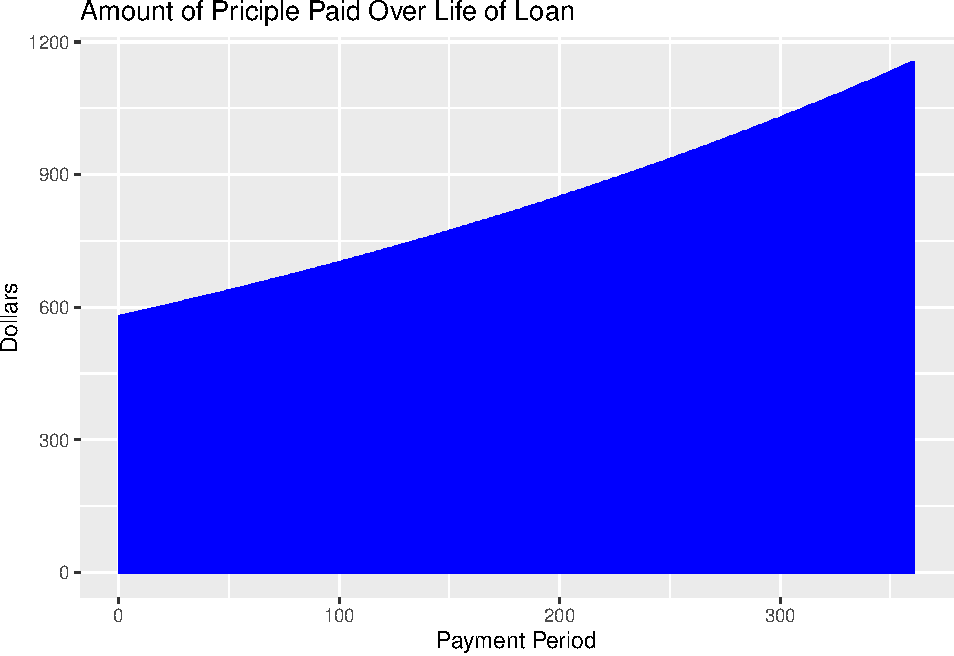
\includegraphics{2020-07-26-time-value-of-money.en_files/figure-latex/unnamed-chunk-4-1.pdf}

\end{document}
